%LLPStartPreview para rodar o pdf com mudancas automaticas


\documentclass{article}
\usepackage{graphicx}
\usepackage{wrapfig}
\usepackage[utf8]{inputenc}
\usepackage[brazil]{babel} % Separacao de silabas em portugues
\usepackage{amsthm} % has proof
\usepackage{amsmath}
\usepackage{listings}
\usepackage{tcolorbox}
\usepackage {tikz}
\usetikzlibrary {positioning}
%\usepackage {xcolor}

\graphicspath{
    {.} % document root dir
    {img/}
}

\renewcommand\refname{Referências}
\newtheorem{theorem}{Teorema}[section]
\newtheorem{corollary}{Corolário}
\newtheorem{lemma}{Lema}

\title{O problema do carteiro chinês}
\author{Carlos Eduardo Ferreira\\Gabriel Fernandes de Oliveira}
\date{}

\begin{document}

\maketitle

\section{As sete pontes de Königsberg}

\begin{wrapfigure}{r}{0.5\textwidth} 
    \centering
    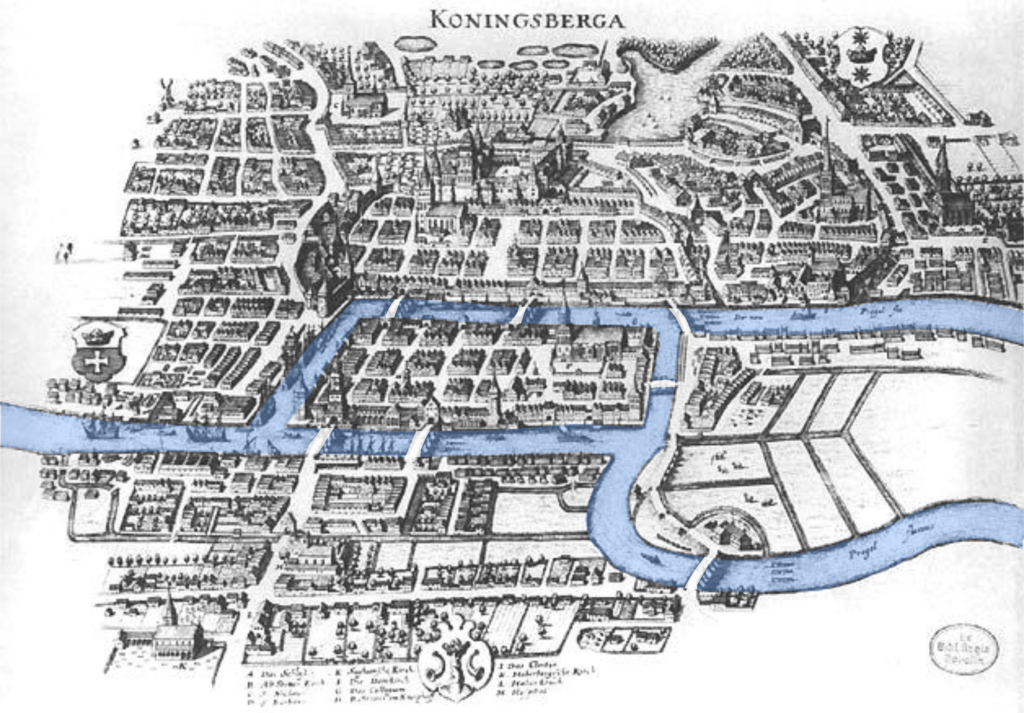
\includegraphics[width=0.5\textwidth]{konigsberg.png}
    \caption{Representação das sete pontes de Königsberg}
\end{wrapfigure}

O problema das sete pontes de Königsberg foi descrito e solucionado pelo matemático Leonhard Euler em 1736, o problema consistia em decidir se seria possível traçar no mapa de Königsberg um trajeto que percorresse cada uma de suas 7 pontes uma única vez, sem repetições.

Euler resolveu esse problema do seguinte modo: 
Primeiramente, ele identificou cada uma das massas de terra do mapa com as letras A, B, C e D.

Em seguida, ele definiu que um trajeto nesse mapa seria descrito por uma sequência dessas letras: por exemplo, "ACD" indicaria o trajeto que se inicia na massa de terra A, move-se para a massa de terra C, usando uma das pontes, e termina na massa D.

\begin{wrapfigure}{l}{0.5\textwidth} 
    \centering
    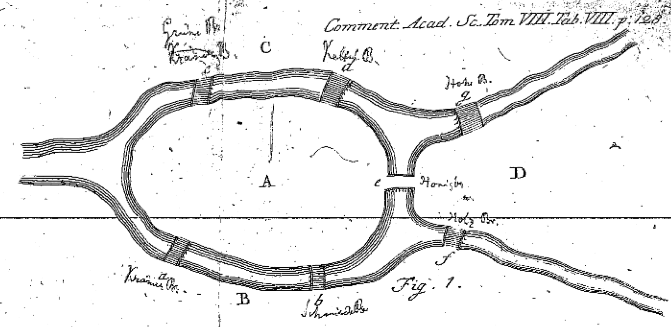
\includegraphics[width=0.5\textwidth]{konigsberg-euler.png}
    \caption{Representação de Euler}
	\label{konigsberg-euler}
\end{wrapfigure}

Euler então começou a definir algumas restrições, assumindo que o problema possuiria alguma solução:

Como o trajeto final deverá passar por todas as 7 pontes exatamente uma vez, isso implica que a sequência de letras que o representa deverá ter tamanho 8.

Além disso, como a massa de terra A possui 5 pontes, necessariamente a letra A aparecerá exatamente 3 vezes na sequência.
A massa B, C e D, no entanto possuem 3 pontes, portanto, suas letras correspondentes deverão aparecer apenas 2 vezes na sequência. 

Chegamos assim a um absurdo, pois inicialmente provamos que a sequência de letras que representa uma solução deveria ter tamanho 8 e depois chegamos que a mesma deveria ter tamanho 9.
Provando assim, por absurdo, que não existe um trajeto como o pedido no enunciado do problema.


Essa obserevação que, aos olhos de hoje, parece muito simples, teve um impacto profundo nas áreas da Matemática e Computação.
A modelagem de Euler, tratando as massas de terra e pontes de forma abstrata foi absoluatmente inovadora e é o embrião da área da teoria dos grafos.


Vamos definir como \textbf{passeio} em um grafo uma sequência finita não vazia $P = \{ v_0, v_1, \dots, v_k\}$, cujos termos são vértices $v_i$ tal que, para todo $i$, $0 \leq i < k$, os vértices $v_{i}$ e $v_{i+1}$ são ligados por uma aresta. 
Os vértices $v_0$ e $v_k$ são a origem e o término de $P$, respectivamente; e os vértices $v_1, v_2, \dots, v_{k-1}$ são chamados vértices internos de P. 

Uma \textbf{trilha} é um passeio sem arestas repetidas. 
Um \textbf{caminho} é um passeio sem vértices repetidos.
Definimos o comprimento de um passeio, denotado por $||P||$, como o número de arestas de $P$.

Um passeio é considerado \textbf{fechado} se sua origem e término são iguais.

Uma trilha fechada é um \textbf{circuito}.

Devido às contribuições de Euler ao problema descrito, chama-se \textbf{trilha euleriana} como uma trilha que passa por todas arestas de um grafo e \textbf{grafo euleriano} como um grafo que possui um circuito euleriana fechada.

Euler modelou essa área da cidade como um grafo, representado na figura \ref{konigsberg-graph}, tratando as pontes como arestas e as massas de terra como vértices.
A partir de tal modelagem e das definições feitas, o problema de Königsberg consiste, em definir se o grafo que representa a cidade possui ou não uma trilha euleriana. 


\begin{wrapfigure}{l}{0.25\textwidth}
    \centering
    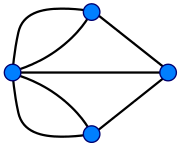
\includegraphics[width=0.25\textwidth]{konigsberg-graph.png}
    \caption{Modelagem de Königsberg como um grafo}
    \label{konigsberg-graph}
\end{wrapfigure}

Apesar de ter recebido grande parte do crédito histórico pelas suas implicações, Euler não provou que qualquer grafo conexo com vértices de grau par era euleriano, essa prova só foi publicada mais de cem anos depois, em 1873, por Carl Hierholzer \cite{hierholzer}, no que se tornou o conhecido Teorema de Euler.


\begin{theorem}[Teorema de Euler ou de Euler-Hierholzer]
    Um grafo é euleriano se, e somente se, é conexo e todos seus vértices possuem grau par.
    \label{euler}
\end{theorem}

Antes de mostrar a prova de tal teorema, primeiramente apresentaremos o seguinte lema:

Seja $\delta(G)$ o grau mínimo de um vértice pertencente a $G$.

\begin{lemma}
	\label{lema}
	Se $G$ é um grafo tal que $\delta(G) \geq 2$, então $G$ possui um circuito.
\end{lemma}

\begin{proof}
	Vamos assumir que um grafo qualquer $G = \{V, A\}$ não possui um caminho fechado. 
	Seja $P$ um caminho de comprimento maximal pertencente a $G$, denominamos $v$ um dos extremos de $P$. 
	Como $P$ é um caminho de comprimento maximal, é impossível, por definição, que $v$ possua uma aresta $vu$ que o ligue a um vértice $u$ não pertencente a $P$.
	
	Como, da premissa, todos vértices possuem grau maior ou igual a 2, isso implica que $v$ possuirá ao menos duas arestas que o ligam a vértices pertencentes a $P$.

	Porém, como $v$ é um vértice extremo de $P$, apenas uma dessas arestas pode pertencer ao caminho $P$. Isso implica que a outra aresta, digamos $vw$, não pertencente a $P$, implica na existência de um caminho fechado.

	Basta tomar o subcaminho entre os vértices $v$ e $w$ pertencente à $P$ juntamente com a aresta $vw$ que teremos um caminho fechado. Chegando assim em uma contradição.

	Demonstra-se assim que $G$ deverá possuir ao menos um caminho fechado dadas as condições do lema.
\end{proof}

Provado tal lema, podemos agora provar o teorema \ref{euler}:

\begin{proof}

Seja $G = \{V, E\}$ o grafo em questão.

($\Rightarrow$) Começamos provando que se um grafo é euleriano então todos seus vértices possuem grau par.

Seja $T$ um circuito euleriano, cuja existência é garantida já que $G$ é euleriano. Analisaremos o grau de um vértice qualquer $v$ de $G$.

Se $v$ não for um vértice extremo de $T$, então sempre que o mesmo aparecer em $T$ ele deverá ser precedido e sucedido de arestas. Indicando assim que $v$ deverá possuir um grau par.

Do contrário, se $v$ for o vértice extremo de $T$ ele necessariamente possui duas arestas, uma ligando-o ao segundo vértice do circuito, e outra o ligando ao penúltimo vértice de $T$. 
Além disso, cada aparição de $v$ como vértice interno de $T$ contabiliza mais duas arestas ao vértice em questão, de modo que $v$ possuirá um grau par ao final.

Sendo assim, se $G$ é euleriano, então todos seus vértices (extremos ou não) possuem grau par, como queriamos demonstrar.\newline

($\Leftarrow$) Agora, provaremos por indução no número de arestas de $G$ que se o grafo for conexo e se todos seus nós possuem grau par, então ele é euleriano.

O caso base da indução é quando não há arestas em $G$. 
O único grafo conexo que respeita tal condição é o grafo que possui apenas um vértice $v$.
Neste exemplo, $\{v\}$ é o circuito euleriano do grafo.

A hipótese de indução é que todo grafo simples, conexo, que possui até $k-1$ arestas e cujos vértices têm grau par é euleriano. 
Seja $G$ um grafo conexo, de vértices de grau par e que possua $k$ arestas, provaremos que ele também deverá ser euleriano.

Como $G$ é conexo, vale que $\delta(G) \geq 1$ e como todos nós de $G$ têm grau par, podemos afirmar que $\delta(G) \geq 2$. 
Sendo assim, pelo lema \ref{lema}, $G$ deverá possuir um circuito $C$.

Se $C$ possui todas arestas de $G$, então $C$ é um circuito euleriano do grafo, finalizando a prova.

Do contrário, aplicamos o seguinte procedimento para constuir um circuito euleriano $\cal{C}$ de $G$:

Retira-se de $G$ as arestas pertencentes a $C$, resultando assim em um grafo $G'$. 
Possivelmente $G'$ será desconexo, por isso definimos que $G'$ será a união de $k$ componenetes conexas $G'_1, G'_2, \dots, G'_k$ disjuntas entre si.

O grau dos vértices dessas componenentes $G'_i$ deverá ser par, já que, ao retirar todas as arestas de um circuito do grafo $G$, diminuimos o grau de um vértice qualquer $v$ em duas vezes o número de aparições do mesmo no circuito. mantendo assim a paridade dos graus. 

Além disso, cada componenete conexa de $G'$ possuirá uma quantidade de arestas menor do que $k$.
Portanto, pela hipótese da indução, cada uma dessas componentes deverá possuir um circuito euleriano próprio. 
Chamaremos de $C_i$ o circuito euleriano da componente $G'_i$.

Ao longo do algoritmo, os circuitos $C_i$ serão adicionados, um a um, ao circuito resultante $\cal{C}$. 
Definimos $\cal{T}$, como o conjunto dos circuitos eulerianos $C_i$ que ainda não fazem parte de $\cal{C}$. 
Inicialmente, $\cal{T}$ é igual ao conjunto $\{C_1, C_2, \dots, C_k\}$.


\[
	C = \{v, v_2, \dots, v_n, v\}
\]

Para cada vértice $u$ de $C$ devemos realizar as seguintes verificações:

\begin{tcolorbox}

Começamos adicionando $u$ ao circuito euleriano $\cal{C}$ que estamos construindo.

Enquanto houver um circuito euleriano $C_i$ pertencente a $\cal{T}$ do qual $u$ faz parte, fazemos o seguinte:


\begin{enumerate}
    \item Representamos $C_i$ como: 
    \[
        C_i = \{u, u_2, \dots, u_l, u\}
    \]

\item Adicionamos ao final de $\cal{C}$ o circuito $C_i$ como representado, exceto pelo primeiro vértice $u$. 

\item Removemos de $\cal{T}$ o circuito $C_i$, indicando que a mesma já foi adicionada a $\cal{C}$.

\end{enumerate}

Repetem-se então as mesmas verificações para os próximos vértices de $C$.
\end{tcolorbox}


Ao final desse procedimento, o conjunto $\cal{T}$ deverá ser vazio, já que toda trilha $C_i$ possui pelo menos um vértice em $C$. Além disso, toda trilha $C_i$ deverá ter sido adicionada à $\cal{C}$ uma única vez, já que logo após adicionar uma trilha à $\cal{C}$ já a removiamos de $\cal{T}$, impedindo que ela fosse adicionada outra vez na trilha euleriana final.

Comprovado o passo da indução, finalizamos a prova do Teorema de Euler por indução.

\end{proof}

\begin{corollary}
    Um grafo possui uma trilha euleriana se, e somente se, é conexo e possui apenas zero ou dois vértices de grau ímpar.
\end{corollary}

\begin{proof}
    Seja $G$ um grafo conexo qualquer. Realizaremos a demonstração para os seguintes casos:
    \begin{enumerate}
        \item $G$ não possui vértices de grau ímpar. Neste caso, $G$ possui, segundo o teorema \ref{euler}, um circuito euleriano, e portanto, uma trilha euleriana.
        
        \item $G$ possui apenas um vértice de grau ímpar. 
			Este caso é impossível de se acontecer, já que a soma do grau de todos vértices deve ser par, impossibilitando assim que apenas um vértice tenha grau ímpar.
        
        \item $G$ possui dois vértices de grau ímpar. 

			Sejam $u$ e $v$ os únicos vértices de $G$ que possuem grau ímpar.
			Adiciona-se uma aresta fictícia ao grafo $G$, a aresta $uv$, fazendo com que tanto $u$ quanto $v$ possuam graus pares. 
			Chamaremos o grafo $G$ acrescido da aresta $uv$ de $G'$.
			Como $u$ e $v$ eram os únicos vértices de grau ímpar de $G$, vale que todos vértices de $G'$ possuirão grau par. 
			Além disso, vale que $G'$ é conexo, pois faz parte da premissa que o grafo original $G$ era conexo.

			Sendo assim, podemos aplicar o teorema \ref{euler}, provando a existência de um circuito euleriano $G'$, que chamaremos de $C$.
            Por ser euleriano, $C$ deverá percorrer a aresta $uv$ inserida, portanto podemos representar $C$ com $u$ e $v$ lado a lado, do seguinte modo:
		
			\[
				C = \{u, v, w_1, w_2, \dots, w_k, u\}
			\]


            Tome, agora, $T$ igual ao circuito $C$ sem seu vértice inicial:

            \[
                T = \{v, w_1, w_2, \dots, w_k, u\}
			\]

            Tal procedimento retira do circuito $C$ a aresta artificial $uv$, transformando-o em uma trilha $T$, que percorre todas arestas de $G`$ exceto $uv$, sendo portanto uma trilha euleriana do grafo $G$.

        \item $G$ possui três ou mais vértices de grau ímpar. 

			Assuma que existe uma trilha euleriana $T$ para $G$. 
			Neste caso, como pelo menos 3 vértices possuem grau ímpar, necessariamente existirá um vértice $v$ que não é nem o primeiro nem o último vértice de $T$.
			Isso implica que todas aparições de $v$ em $T$ são internas ao caminho, ou seja, toda aparição de $v$ será precedida e sucedida de arestas ligadas a $v$.
			Como estamos tratando de uma trilha euleriana, sabemos que todas arestas adjacentes a $v$ estão presentes em $T$ uma única vez. 
			Mas como todas arestas de $v$ devem aparecer em pares (precedendo e sucedendo $v$), isso implica que o grau de $v$ deverá ser par.
			Contradizendo a premissa.

			Por essa contradição provamos que $G$ não possuirá trilha euleriana se tiver três ou mais vértices de grau ímpar.
    \end{enumerate}
\end{proof}


%Segue agora uma implementação de um algoritmo que encontra o circuito euleriano de um grafo dado que o mesmo possui um circuito euleriano:

%\lstinputlisting[language=c++]{euler_cycle.cpp}


\section{O problema do Carteiro Chinês}

Com o passar dos anos, a área de teoria dos grafos se desenvolveu muito, tratando dos mais variados tipos de problemas.

Em 1962, mais de 200 anos após Euler descrever sua solução para o problema de Konigsberg, o matemático chinês Meigu Guan publicou um estudo que generalizava ainda mais o problema dos grafos eulerianos. 
Esse problema foi denominado Problema da Inspeção de Rotas, ou, como também é conhecido hoje: Problema do carteiro chinês.
A ideia desse problema é encontrar um passeio fechado que visite toda aresta de um grafo conexo pelo menos uma vez. 
A grande diferença aqui é que as arestas podem ser repetidas, ou seja, usadas mais de uma vez no trajeto final.

O nome do problema está relacionado a um problema que carteiros encontram no planejamento de suas rotas: dada uma cidade com várias ruas de diferentes comprimentos e um posto de carteiros, encontrar a menor rota que um carteiro deve percorrer de modo a poder entregar cartas em todas as ruas da cidade e voltar ao posto de carteiros no fim de sua rota.

\begin{wrapfigure}{l}{0.3\textwidth} 
    \centering
    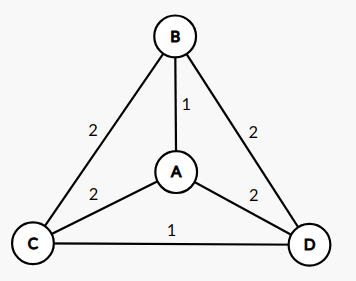
\includegraphics[width=0.3\textwidth]{graph.png}
	\caption{Exemplo de grafo}
	\label{graph}
\end{wrapfigure}

Por exemplo, para a figura \ref{graph}, um passeio fechado de custo ótimo seria: \[ \{A, B, D, C, A, D, C, B, A\} \], sendo este um caminho fechado de custo 12.
Neste exemplo foi necessário que as arestas $AB$ (ou $BA$) e $DC$ (ou $CD$) fossem percorridas duas vezes no passeio, porém nem sempre é necessária esta repetição.

No caso em que o grafo tratado é euleriano, a resposta para o problema do carteiro chinês é justamente o circuito euleriano do grafo.
Nos outros casos, sendo o grafo conexo, o procedimento que seguiremos será similar a realizar a cópia de algumas arestas do grafo de modo a torná-lo euleriano, ou seja, adicionar duplicatas de arestas até que todos os vértices possuam grau par.

Discutiremos nas seções a seguir a solução para o problema em questão com base nas especificidades do grafo do problema:

\subsection{Grafos não direcionados}

Analisaremos o caso em que o problema é modelado a partir de um grafo $G(V, E)$ simples, conexo e com arestas não direcionadas.

Um circuito Euleriano é um circuito que percorre todas arestas de $G$ exatamente uma vez. 
Já um circuito $C$ qualquer que resolva o problema do carteiro chinês deverá percorrer cada aresta de $G$ pelo menos uma vez.
Seja $1 + x_e$ o número de vezes que uma aresta $e \in E$ é percorrida na solução $C$ do problema do carteiro chinês (PCC).

Se $G$ é euleriano, então a solução para o PCC é o próprio circuito euleriano do grafo.

Do contrário, definimos $G'$ como o grafo formado por $G$ adicionado de $x_e$ cópias de cada aresta $e \in E$. 
Isto é, cada aresta $e$ de $G$ aparecerá em $G'$ $1 + x_e$ vezes.
Deste modo, o grafo $G'$ será euleriano, e portanto a trilha euleriana de $G'$ corresponderá à solução do PCC para o grafo $G$.

Sendo assim, podemos separar a solução do PCC em duas partes: Encontrar o valor ótimo de $x_e$ para o problema descrito e, em seguida, encontrar um circuito euleriano no grafo $G'$ construído.

Resolveremos a primeira parte do problema com um algoritmo de emparelhamento.

%Seja $E(v)$ o conjunto de arestas ligadas ao vértice $v \in V$, e seja $c_e$ o custo de se percorrer uma aresta $e \in E$, que deverá ser não-negativo.

%Encontrar uma solução ótima para o PCC é equivalente a encontrar os valores inteiros e não negativos $x_e$ tal que $\sum_{e\in E(u)}(1 + x_e) \equiv 0 \mod 2$ para todo $u \in V$, minimizando o valor de $\sum_e c_ex_e$.

\begin{lemma} 
    \
    Para todo grafo simples e conexo, existirá uma solução ótima do PCC em que cada aresta é copiada no máximo 1 vez, ou seja que $x_e$ valerá apenas 0 ou 1. 
\end{lemma}

\begin{proof}
    Seja $x$ uma solução ótima do PCC para um grafo $G$, sabemos que $x$ deverá possuir valores inteiros não negativos, além disso, sabemos que o grafo $G'$, induzido por $x$, deverá ser euleriano e que o valor de $\sum_e c_ex_e$ será mínimo.

    Seja $x^*$ um vetor definido do seguinte modo:

    \[  x^*_e = x_e \bmod 2    \]

    Como o grafo $G'$ induzido por $x$ era euleriano, o grafo $G^*$ induzido por $x^*$ também deverá ser euleriano, pois a paridade dos vértices em ambos grafos é a mesma, e também pois tanto $G'$ quanto $G^*$ possuem $G$, que é conexo, como um subgrafo, e portanto também são conexos.
    
    Pela definição, $G^*$ usa um número menor ou igual de arestas duplicadas que $G'$, fazendo com que o seguinte se mantenha: $\sum_e c_ex^*_e \leq \sum_e c_ex_e$.

    No entanto, como $x$ consistia de uma solução ótima, sabemos que $\sum_e c_ex_e$ deverá ser mínimo, e portanto, $\sum_e c_ex^*_e = \sum_e c_ex_e$. 


    Finalmente, como $x$ era uma solução ótima o valor de $\sum_e c_ex_e$ deverá ser mínimo, sendo assim, deve valer que $\sum_e c_ex^*_e = \sum_e c_ex_e$, provando assim a otimalidade de $x^*$, uma solução ótima que respeita as condições do lema.
\end{proof}

\begin{lemma}
    \label{lemma-pcc}
    O conjunto de arestas duplicadas de uma solução ótima para o problema consistirá de um conjunto de caminhos aresta-disjuntos entre vértices de grau ímpar.
\end{lemma}

\begin{proof}
    Seja $x$ uma solução ótima do PCC para um grafo $G(V, E)$ em que cada aresta é copiada no máximo 1 vez, cuja existência é garantida pelo lema \ref{lemma-pcc}.
    Realizaremos uma prova deste lema por indução no número de arestas duplicadas de $G$, ou seja, em $\sum_e x_e$, para toda aresta $e \in E$. 

    O caso base dessa indução é quando $\sum_e x_e = 0$. 
    Neste caso, o conjunto de areastas duplicadas será vazio, valendo então a propriedade do lema.

    A hipótese de indução será que a propriedade do lema vale para uma soma $\sum_e x_e < k$, com $k > 0$.

    Analisaremos agora o caso em que $\sum_e x_e = k$, com $k > 0$.

    Vamos assumir que $G$ não possui nenhum vértice de grau ímpar, isso implica na existência de um circuito $C$ de arestas com $x_e = 1$, como, por exemplo, o representado na figura \ref{pcc-case2}.  
    
    Se este for o caso, podemos simplesmente fazer com que $x_e = 0$ para toda aresta $e$ pertencente ao circuito $C$. 
    Esse procedimento deleta arestas duplicadas desnecessárias à uma solução ótima. 

    Podemos 

    \begin{figure}
        \centering
        \begin{tikzpicture}[auto,node distance=3cm, every loop/.style={},thick,main node/.style={circle,draw,font=\sffamily\Large}]
            \node[main node] (5) {5};
            \node[main node] (1) [below left of=5]{1};
            \node[main node] (2) [below of=1] {2};
            \node[main node] (4) [below right of=5] {4};
            \node[main node] (3) [below of=4] {3};

          \path[every node/.style={font=\sffamily\small}]
            (5) edge node [above] {0} (1)
            (5) edge node [above] {0} (4)
            (1) edge node [above] {0} (4)
            (2) edge node [right] {1} (1)
            (3) edge node [above] {1} (2)
            (4) edge node [left] {1} (3)
            ;
        \end{tikzpicture}
        \caption{Possível estrutura em grafo com vértices de grau ímpar}
        \label{pcc-case1}
    \end{figure}
    \begin{figure}
        \centering
        \begin{tikzpicture}[auto,node distance=3cm, every loop/.style={},thick,main node/.style={circle,draw,font=\sffamily\Large}]
            \node[main node] (1) {1};
            \node[main node] (2) [below of=1] {2};
            \node[main node] (4) [right of=1] {4};
            \node[main node] (3) [below of=4] {3};

          \path[every node/.style={font=\sffamily\small}]
            (1) edge node [above] {1} (4)
            (2) edge node [right] {1} (1)
            (3) edge node [above] {1} (2)
            (4) edge node [left] {1} (3)
            ;
        \end{tikzpicture}
        \caption{Caso em que o grafo tratado não possui vértices de grau ímpar}
        \label{pcc-case2}
    \end{figure}

\end{proof}




% TODO: Finalizar solução para grafo não direcionado. Fazer exemplo.


A solução se baseia em criar um novo grafo $G'(V', E')$. 
$V'$ é definido como o subconjunto de vértices de $V$ que possuem um grau ímpar em $G$. 
Já $E'$ será definido como o conjunto de arestas entre todo par de vértices de $V'$, dado que uma aresta entre dois vértices $u$ e $v$ quaisquer terá o custo igual ao custo do menor caminho entre $u$ e $v$ no grafo original $G$.


\textbf{Solução:} 
\begin{enumerate}
    \item Criar um grafo completo ligando todos vértices $u, v$ que possuirem grau ímpar com arestas de custo igual ao menor caminho entre $u$ e $v$. 
    \item Rodar algoritmo de emparelhamento perfeito de custo mínimo (Húngaro com otimização do Edmonds e Karp, $\mathcal{O}(n^3)$).
\end{enumerate}


\textbf{Observações:}
\begin{itemize}
		\item Pelo ``Lema do aperto de mão'' é garantido que haverá um número par de vértices de grau ímpar.
		\item Essa solução não se aproveita do grafo ser esparso, há outra formulação do Edmonds e Johnson que leva isso em consideração.
		\item Um problema similar é o de cobrir todas arestas com ciclos simples, de modo que o comprimento total dos ciclos é minimizado. Para grafos planares esses problemas são equivalentes.
	\end{itemize}

	\section{Directed CPP}

	O grafo deverá ser fortemente conexo.\\

	\textbf{Solução:}
	\begin{enumerate}
		\item Criar um grafo $P, Q$-bipartido completo. $P$ deve conter todos os vértices do grafo original com excesso de grau de entrada, e $Q$ deve conter todos vértices com excesso de grau de saída. que possuem valores diferentes de grau de entrada e saída. O custo das arestas entre $P$ e $Q$ deverá ser igual ao custo do menor caminho entre os dois vértices que a mesma liga.
		\item Modelar uma rede de fluxo: vértices de $P$ recebem um excesso igual a diferença do grau de entrada pelo grau de saída, vértices de $Q$ recebem uma demanda igual a diferença do grau de saída pelo grau de entrada. 
		\item Rodar um algoritmo de fluxo de custo mínimo. 
	\end{enumerate}

	\textbf{Observações:}
	\begin{itemize}
		\item Modelagem de fluxo com arestas de capacidade unitária, aumentando a velocidade do algoritmo.
	\end{itemize}

	\section{Mixed CPP}

	NP-hard, mesmo se $G$ for planar e se todos $c_{ij}$ forem iguais.

	\section{Windy Postman Problem}

	NP-hard

	Se todo ciclo do grafo tem o mesmo custo em ambos sentidos, transforma a aresta entre $i$ e $j$ de custos $c_{ij}$ e $c_{ji}$ em uma aresta não direcionada com custo $\frac{c_{ij} + c_{ji}}{2}$. Essa transformação reduz o problema de a um CPP não direcionado, que tem solução polinomial, porém para isso é necessário checar se todo ciclo tem o mesmo custo nas duas direções.

	\section{Hierarchical Postman Problem}

	NP-hard 

	Seja $P = \{A_1, A_2, \dots, A_k\}$ uma partição do conjunto de arestas $A$. Determinar um caminho em $G$ de custo mínimo que sai de um vértice $s$ e atinge um vértice $t$, respeitando uma hierarquia das arestas. O caminho só poderá possuir uma aresta pertencente a $A_j$ se o caminho passar anteriormente por todas arestas pertencentes a $A_i$, se $i < j$.


	\section{Anotações}

	\begin{itemize}
		\item Todo mixed CPP pode ser transformado em um WPP.
	\end{itemize}

	\medskip

	\begin{thebibliography}{9}
	\bibitem{konigsberg} 
	Euler, Leonhard
	\textit{Solution problematis ad geometriam situs pertinentis}. 
	Comment. Acad. Sci. U. Petrop 8, 128–40, 1736.

	\bibitem{hierholzer}
	Hierholzer, Carl
	\textit{``Über die Möglichkeit, einen Linienzug ohne Wiederholung und ohne Unterbrechung zu umfahren''}, 
	Mathematische Annalen, 6 (1): 30–32, doi:10.1007/BF01442866, 1873.
	\end{thebibliography}
 
\end{document}

\end{document}
